\documentclass[tikz, preview]{standalone}

\usepackage{amsfonts, amsthm, amssymb, amsmath, stmaryrd, etoolbox}
\usepackage{tikz}
\usetikzlibrary{matrix,arrows}

\begin{document}
\[
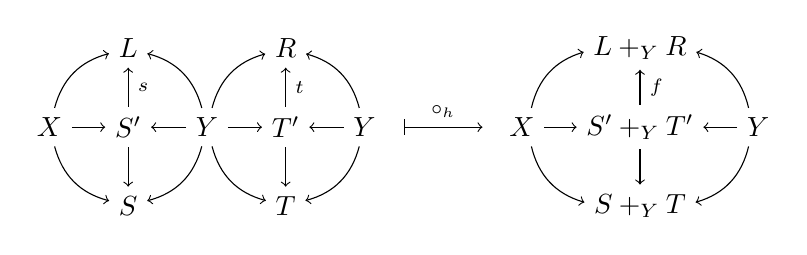
\begin{tikzpicture}
\node (X) at (-5,0) {$X$};
\node (Y) at (-3,0) {$Y$};
\node (Z) at (-1,0) {$Y$};
\node (L) at (-4,1) {$L$};
\node (S') at (-4,0) {$S'$};
\node (S) at (-4,-1) {$S$};
\node (R) at (-2,1) {$R$};
\node (T') at (-2,0) {$T'$};
\node (T) at (-2,-1) {$T$};
%
\draw [->] (X) edge[bend left=30] (L);
\draw [->] (X) edge (S');
\draw [->] (X) edge[bend right=30] (S);
\draw [->] (Y) edge[bend right=30] (L);
\draw [->] (Y) edge (S');
\draw [->] (Y) edge[bend left=30] (S);
\draw [->] (Y) edge[bend left=30] (R);
\draw [->] (Y) edge (T');
\draw [->] (Y) edge[bend right=30] (T);
\draw [->] (Z) edge[bend right=30] (R);
\draw [->] (Z) edge (T');
\draw [->] (Z) edge[bend left=30] (T);
\draw [font=\scriptsize,->] (S') edge node[right] {$s$} (L);
\draw [->] (S') edge (S);
\draw [font=\scriptsize,->] (T') edge node[right] {$t$} (R);
\draw [->] (T') edge (T);
%-------------------------------
\draw [font=\scriptsize,|->] (-0.5,0) -- node[above] {$\circ_h$} (0.5,0);
%-------------------------------
\node (X) at (1,0) {$X$};
\node (Y) at (4,0) {$Y$};
\node (L) at (2.5,1) {$L+_YR$};
\node (L') at (2.5,-1) {$S+_YT$};
\node (Spb) at (2.5,0) {$S'+_YT'$};
%
\draw [->] (X) edge[bend left=30] (L);
\draw [->] (X) edge[] (Spb);
\draw [->] (X) edge[bend right=30] (L');
\draw [->] (Y) edge[bend right=30] (L);
\draw [->] (Y) edge[] (Spb);
\draw [->] (Y) edge[bend left=30] (L');
\draw [font=\scriptsize,->] (Spb) edge node[right] {$f$} (L);
\draw [->] (Spb) edge[] (L');
\end{tikzpicture}
\]
\end{document}
